\documentclass{template/openetcs_article}
%\documentclass{article}
%\usepackage[ascii]{inputenc}
%\usepackage[T1]{fontenc}
\usepackage[english]{babel}
\usepackage{amsmath}
\usepackage{amssymb,amsfonts,textcomp}
\usepackage{array}
\usepackage{supertabular}
\usepackage{hhline}
\usepackage{graphicx}
\makeatletter
\newcommand\arraybslash{\let\\\@arraycr}
\makeatother
\setlength\tabcolsep{1mm}
\renewcommand\arraystretch{1.3}
\newcounter{Ilustracin}
\renewcommand\theIlustracin{\arabic{Ilustracin}}
\title{openETCS}

%\setcounter{tocdepth}{3}
\usepackage{float}
\usepackage{hhline}
\usepackage{booktabs}
\usepackage{multirow}
\usepackage{color, colortbl}
\definecolor{myblue}{rgb}{0.6,.6,1}
\definecolor{mydarkblue}{rgb}{0,0,0.5}
\definecolor{mylightblue}{rgb}{0.8,0.8,1}
\usepackage{hyperref}
\hypersetup{colorlinks=true, linkcolor=mydarkblue, urlcolor=mydarkblue}

\usepackage[textwidth=2.7cm,textsize=scriptsize,linecolor=green!40,backgroundcolor=green!40]{todonotes}

\newcounter{mycommentcounter}
\newcommand{\mycomment}[2][]
{
\refstepcounter{mycommentcounter}%
\todo[color={red!100!green!33}]{
\textbf{[\uppercase{#1} \themycommentcounter]:} #2}
}


\usepackage{lipsum,url}
\graphicspath{{./template/}{.}{./images/}}
\begin{document}
\frontmatter
\project{openETCS}

%Please do not change anything above this line
%============================
% The document metadata is defined below

%assign a report number here
\reportnum{OETCS/WP1/Revision and Review processes}

%define your workpackage here
\wp{Work-Package 1: ``Management''}

%set a title here
\title{Project Quality Assurance Plan - Presentation of the Revision and Review Processes}

%set a subtitle here
%\subtitle{A template for short document. Adapted from report template.}

%set the date of the report here
\date{\today}

%define a list of authors and their affiliation here

\author{SQS}

\affiliation{Avda. Zugazarte 8,6\\
  48930 Getxo \\
  Vizcaya, España}


% define the coverart
\coverart[width=350pt]{openETCS_EUPL}

%define the type of report
\reporttype{Description of work}




%=============================
%Do not change the next three lines
\maketitle
\tableofcontents
%\listoffiguresandtables
\newpage
%=============================

% The actual document starts below this line
%=============================


%Start here



%\begin{document}


\section*{Document History}

\begin{flushleft}
%\tablefirsthead{\hline Version & Date & Chapters modified & Reason & Name\\}

\tablehead{\hline \rowcolor{myblue} Version & Date & Chapters modified & Reason & Name\\}

\tabletail{}
\tablelasttail{}
\begin{supertabular}{m{1.1cm}m{1.8cm}m{2cm}m{7cm}m{2cm}lp{6cm}|}
\hline
0.0.1 &
23.05.2013 &
All &
First version &
SQS
\\
\end{supertabular}
\end{flushleft}

\newpage

\section{Introduction}
Two different processes have been identified:
\begin{itemize}
\item \underline{\textbf{Revision Process}} - The OpenETCS committers are invited to perform a revision of the contents of a document. The committers can edit the document, writing complete sections or making changes directly in it (LaTex, todonotes and Smartgit tools). The author(s) shall support the whole process answering questions and resolving conflicts. Once the author(s) and committers are satisfied with the results, the Product owner shall confirm and approve or reject and request more changes to the revised document. Finally, the approved document is pushed into the corresponding GitHub repository.
\item \underline{\textbf{Review Process}} - Any person involved in the GitHub communnity and/or the OpenETCS project is invited to participate in a Review Process. They shall not edit the document but send comments and suggestions creating the corresponding issues in the {\it Issue Tracker} tool. Once the deadline has arrived, the author(s) shall collect the comments and make the changes they consider appropriate. Any doubt shall be answered by the reviewers using the issue threads opened and in case of conflicts the collaboration of the Product owner may be required. The process may be launched after a Revision Process ends, there are relevant issues reported for a release or whenever the Product owner considers appropriate. 
\end{itemize}

The following diagram presents the Flow of the Revision/Review processes.

\begin{figure}[H]
\centering
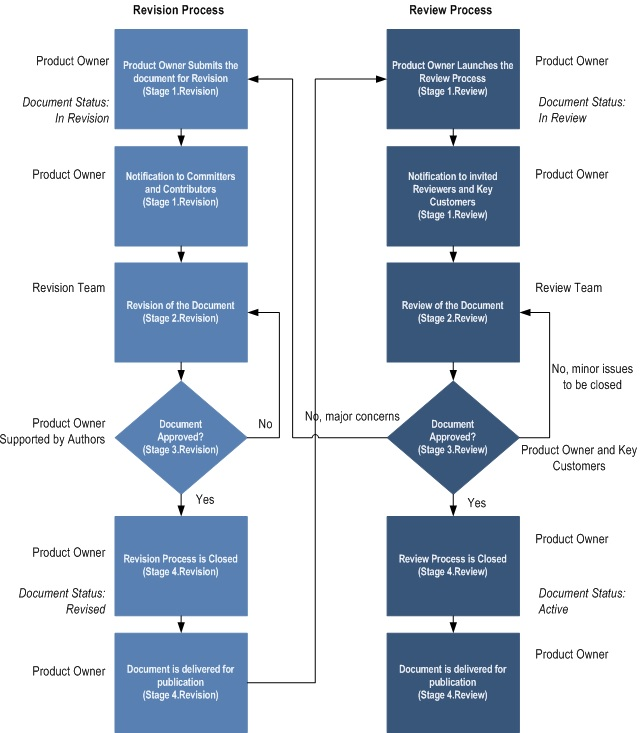
\includegraphics{./figures/RevisionReviewProcess.JPG}
\caption{Revision-Review Processes flow}
\end{figure}

In the following sections a summary of both processes is provided. 

\section{Revision Process}
The Revision of a document implies the {\it\underline{reworking}} of a document following a set of steps that are performed in sequential order. A typical scenario shall include one or more authors creating a document that is then revised by a specific number of registered committers and finally approved by a specific individual.

The document revision cycle consists on several stages. After the document is created and confirmed its first version, it is pushed to the GitHub repository and made available to the committers for revision either concurrently or sequentially. 

This process requires collaboration between the committers and the autor(s). After all of the committers’ comments, suggestions, and changes made directly to the document have been accepted by the author(s), the revised document shall be approved, or not, by the Product Owner. The Product owner can be one of the authors or the Project Leader, and who is going to play this roles shall be decided at the beginning of the Revision process. 

More changes can be requested by the Product owner and he/she shall be the responsible for making final decisions and solving conflicts between the commiters and/or the author(s).

When approved, the document with the changes is pushed to the corresponding GitHub repository and its availability notified via the Issue tracker. 

Then, the process can be closed and the corresponding Revision Cycle branch merged to the {\it master branch}.

In order to be truly effective, the Revision process must take full advantage of the editing and document generation tools available in the project (LaTex, Smartgit, todonotes, PDF creator, etc.), including the use of GitHub to have always a version with the changes included remotely (not only in local) and accessible to all the committers and author(s). The process requires that all the committers involved have the appropriate knowledge in using and managing these tools.

From this moment, the document is in the 'Version revised' state and it can be put under review.

The stages involved in the process are shown in the next diagram:

\begin{figure}[H]
\centering
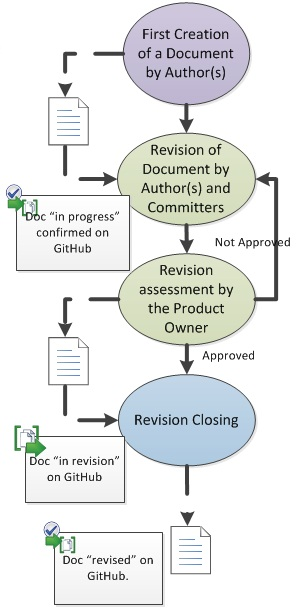
\includegraphics{./figures/RevisionProcess.JPG}
\caption{Stages of the Revision Process}
\end{figure}

\section{Review Process}
The Review of a document implies {\it\underline{looking at something}}, so it shall be strictly limited to reading a document and giving comments using the GitHub {\it Issue Tracker} tool. 

A typical scenario shall include the product owner makes the document available in GitHub and creates an issue calling for reviewers. A deadline is set so at the end of the period all the issues reported via the {\it Issue Tracker} are collected. 

The author(s) assess the comments and suggestions made and decide whether they shall be considered or not, justifying each decision. In this way only the author(s) shall edit the document and not the reviewers, and any question or doubt that appears shall be answered by the reviewers through the {\it Issue Tracker} tool. Because of this, the author(s) should have enough time to implement the changes and ask questions to the reviewers.

A Review process could be started not only after a Revision Process has been done, but also in other contexts. \underline{The process shall be started once the following situations have been identified}:

\begin{itemize}
\item After a Revision Process has finished
\item There is a release of a document and in the {\it Issue Tracker} there are a set of relevant issues to that release. A Review process shall be started to collect more issues.
\item There is a special situation because of that the product owner considers to begin a Review Process 
\end{itemize}

This process requires active involvement of the community, reviewers with technical knowledge in several subjects included in the document or some expertise in the project. Any person of the community interested in participate shall provide a brief explanation of his/her expertise and skills so its collaboration could be adequately assessed.

Finally, the Product owner shall decide whether the document deserves an approval or not. And then, there are \underline{three possible situations for the closing}:

\begin{itemize}
\item For each Review Process that finishes with an approval, a new Release shall be generated and pushed into GitHub.
\item There are minor changes pending to be implemented because the modifications made are not enough to close the reported issues. The author(s) shall complete the task.
\item The issues found have reveal that the document needs further improvements, so it has not been approved as release and a new Revision Cycle shall begin, so the author(s) and selected committers can fix the problems identified and generate a more complete version of the document. Then, and with the version revised, a new Review process shall be addressed. 
\end{itemize}

The stages involved in the process are shown in the next diagram:

\begin{figure}[H]
\centering
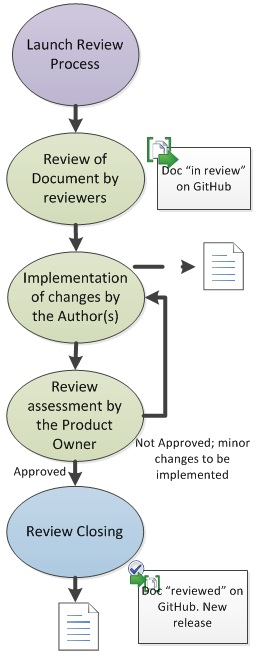
\includegraphics{./figures/ReviewProcess.JPG}
\caption{Stages of the Review Process}
\end{figure}

\end{document}
